%!TEX root = ../dokumentation.tex

\chapter{CAN-Bus}
Der Begriff CAN steht für Controller Area Network.
Mit der zunehmenden Elektronisierung im Automobilbereich kam die Notwendigkeit auf, verschiedene Steuergeräte zu vernetzen.
Mit dem CAN-Bus wurde von der Robert Bosch GmbH ein Bussystem entwickelt, dass erstmals 1990 in Serie im Mercedes-Benz W140 eingesetzt wurde.
Durch seine vielen Vorteile hat sich diese Art des Busses schnell durchgesetzt und wird seitdem flächendeckend in der Automobilbranche verwendet.
Auch heute ist CAN noch der Standard für die Vernetzung von Steuergeräten im Kraftfahrzeugbereich.
Deshalb wurde es auch von der \ac{ISO} und der SAE (Firma für Standardisierung im Automobilbereich) für den Datenaustausch in Kraftfahrzeugen standardisiert.
Es gibt mehrere Versionen des CAN-Bus. Dazu zählt CAN2.0, Single Wire CAN, Low Power CAN, CAN FD und CAN XL.
Mit TTCAN wurde auch ein zeitbasiertes Protokoll eingeführt. 
Can 2.0 kann außerdem in Lowspeed CAN (CAN-B) und in Highspeed CAN (CAN-C) unterschieden werden. 
CAN-B wird hauptsächlich im Komfort- und Karosseriebereich eingesetzt, da dort die Geschwindigkeit von 5kBit/s bis 125kBit/s meist ausreicht. 
Für Geschwindigkeiten von 125kBit/s bis 1Mbit/s wird ein Highspeed-CAN-Bus verwendet.
Dies wird größtenteils für Echtzeitanforderungen beim Antriebsstrang eingesetzt. 

%\begin{figure}[!htbp]
%    \centering
%    \includegraphics[width=0.5\linewidth]{own/CAN/VernetzungVonSteuergeräten_BBA92.png}
%    \caption{Grafik Vernetzung von Steuergeräten, Quelle: \cite{BAA2011, S.92}}
%    \label{fig:VernetzungVonSteuergeraeten}
%\end{figure}

\begin{figure}
    \centering
    \begin{minipage}{.5\textwidth}
      \centering
      \includegraphics[width=0.7865\linewidth]{own/CAN/VernetzungVonSteuergeräten_BBA92.png}
    \caption{Grafik Vernetzung von Steuergeräten,\\Quelle: \cite{BAA2011, S.92}}
    \label{fig:VernetzungVonSteuergeraeten}
    \end{minipage}%
    \begin{minipage}{.5\textwidth}
      \centering
      \includegraphics[width=0.705\linewidth]{own/CAN/Störungsfilterung_BAA94.png}
            \caption{Grafik Vernetzung von CAN Steuergeräten, Quelle: \cite{BAA2011, S.94}}
            \label{fig:Stoerungsfilterung}
    \end{minipage}
    \end{figure}

\section{Übertragungssysteme}

    \subsection{Logische Buszustände und Kodierung}
    Es gibt zwei Zustände, mit denen die Informationsbits übertragen werden.
    Der dominante Zustand stellt eine binäre 0 dar, während der rezessive Zustand eine binäre 1 darstellt.
    Der dominante Zustand ist in der Lage, den rezessiven Zustand zu überschreiben.
    Die Kodierung beim CAN-Bus geschieht nach dem NRZ-Verfahren (Non-Return-To-Zero), welches beschreibt, dass zwischen zwei gleichwertigen Übertragungszuständen nicht zwangsweise ein Nullzustand herrschen muss.
    Zum Senden und Empfangen, werden die logischen Zustände in Binärwerte gerechnet und den CAN-Controller gesendet.
    
    \subsection{Leitungsarten}
        \subsubsection{Zweidrahtleitung}
        Prinzipiell kann für den CAN-Bus jedes beliebige Übertragungsmedium verwendet werden, auf dem es möglich ist, dominante und rezessive Zustände zu übertragen.
        Meist wird eine verdrillte Zweidrahtleitung verwendet, die galvanisch gekoppelt ist. Diese ist kostengünstig und nicht so schwer wie eine stark isolierte Leitung.
        Dadurch, dass die Magnetfelder der zwei Leitungen gegenläufig sind, gleichen sich die Störimpulse der Leitungen aus.
        Es wird auf die zwei Leitungen, CAN\_L (CAN-Low Leitung) und CAN\_H (CAN-High Leitung) eine symmetrische und differenzierte Datenübertragung durchgeführt.
        Dabei werden die Bits unter der Verwendung von unterschiedlichen Spannungen auf die Leitungen übertragen.
        Dadurch reduziert sich die Empfindlichkeit gegenüber Gleichtaktstörungen (Störungen auf beiden Leitungen), da sich diese rechnerisch ausfiltern lassen.
        Dies ist allerdings nur der Fall, wenn sich die Störung auf beide Leitungen gleich auswirkt.
        Ist dies nicht der Fall, hat das System ein Differenzproblem.
        Außerdem kann man das eigene Abstrahlverhalten bei hohen Baudraten durch zusätzliche Schirmung der Leitung erreichen.

        %\begin{figure}[!htbp]
        %    \centering
        %    \includegraphics[width=0.5\linewidth]{own/CAN/Störungsfilterung_BAA94.png}
        %    \caption{Grafik Vernetzung von CAN Steuergeräten, Quelle: \cite{BAA2011, S.94}}
        %    \label{fig:Stoerungsfilterung}
        %\end{figure}
        
        \subsubsection{Eindrahtleitung}
        Zum Einsparen einer zweiten Leitung ist es möglich die Kommunikation über eine Leitung stattfinden zu lassen.
        Dadurch müssen allerdings alle Busteilnehmer über eine gemeinsame Masse verfügen, weshalb dies nur bei räumlich begrenzter Ausdehnung möglich ist.
        Zudem ist das das Ausfiltern von Störimpulsen nicht möglich und die Eindrahtleitung anfälliger gegenüber Störeinstrahlung.
        Dadurch muss ein höherer Pegelhub gewählt werden, was im Gegenzug die eigene Störabstrahlung erhöht, weshalb die Flankensteilheit verringert werden muss.
        Dadurch wird die Übertragungsgeschwindigkeit begrenzt, weshalb eine Eindrahtleitung nur bei Lowspeed CAN im Bereich der Karosserie und Komfortelektronik eingesetzt wird.
        Die Möglichkeit des Betriebs über eine Leitung bedeutet allerdings auch, dass ein Zweidrahtsystem, wenn auch nur eingeschränkt, auch bei Ausfall einer der Leitungen funktionsfähig bleibt. 

    \subsection{Spannungspegel}
    Die Spannungspegel auf den Leitungen werden vom CAN-Transceiver anhand der ihm übergebenen Bitströme gesetzt.
    Highspeed-CAN und Lowspeed-CAN verwenden jeweils unterschiedliche Spannungspegel.
    Die einzelnen Spannungen können anhand von Abbildung \ref{fig:Spannungspegel} abgelesen werden. 
    \begin{figure}[!htbp]
        \centering
        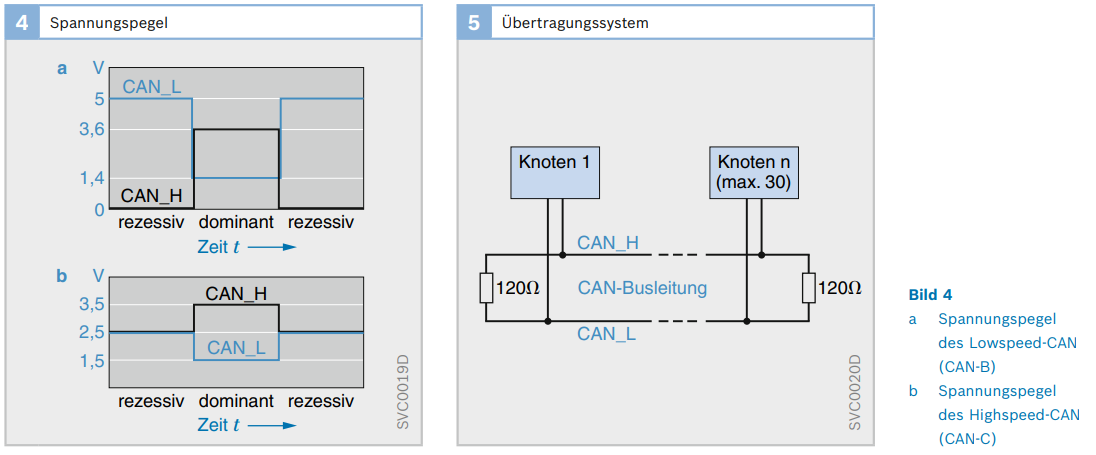
\includegraphics[width=0.8\linewidth]{own/CAN/Spannungspegel_BBA95.png}
        \caption{Grafik Spannungspegel CAN, Quelle: \cite{BAA2011, S.94}}
        \label{fig:Spannungspegel}
    \end{figure}
    
        \subsubsection{Reflexionsfreier Abschluss}
        Damit die Reflexion am Ende einer Leitung gedämpft wird, werden die Busleitungen an beiden Enden mit einem Widerstand von $120 \Omega$ abgesichert.
        Oft werden auch zwei $60 \Omega$ Widerstände verwendet um die Reflexion kontrolliert, mit einem Kondensator mit einer Kapazität von wenigen nF, auf Masse abzuleiten.

    \subsection{Grenzwerte}
    Damit die Auswertung der gesendeten Bits erfolgreich ist, muss das Signal am Abtastzeitpunkt bei jedem Knoten innerhalb einer Bitzeit ungestört vorhanden sein.
    Verzögerungen ergeben sich aus Signallaufzeiten, weshalb die zulässige Übertragungsrate eines Busses von der Gesamtlänge des Bussystems abhängig ist.
    Eine Anzahl von bis zu 30 Netzknoten ist ohne Probleme realisierbar.
    \begin{figure}[!htbp]
        \centering
        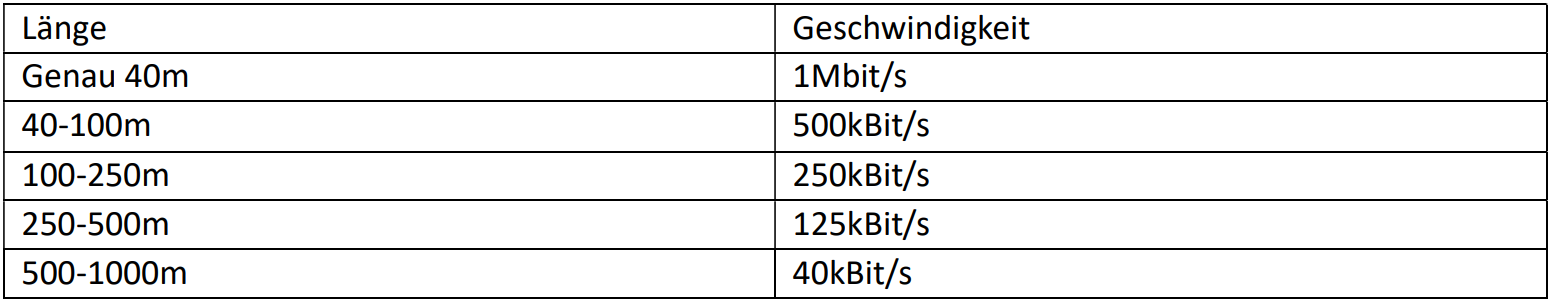
\includegraphics[width=1\linewidth]{own/CAN/Geschwindigkeiten.png}
        \caption{Tabelle Geschwindigkeiten Highspeed-CAN, anhand Quelle: \cite{BAA2011, S.95}}
        \label{fig:Geschwindigkeiten}
    \end{figure}

\section{CAN-Protokoll}
    \subsection{Protokollschichten}
    Zusammenhängende Aufgaben werden beim CAN-Protokoll in thematischen Schichten beschrieben.
    Diese können in das OSI-Modell eingeordnet werden, worauf in diesem Vortrag allerdings nicht weiter eingegangen wird.
    Die oberste Schicht ist die Application-Layer (Anwendungsschicht), in der sich Informationen in Datenstrukturen befinden, die von der Anwendung verwendet werden. 
    Der Object-Layer (Objektschicht) ist für die Verwaltung von Nachrichten zuständig.
    Dieser entscheidet, welche Nachricht zu welchem Zeitpunkt versendet werden soll, und führt die Akzeptanzprüfung durch.
    Darunter folgt der Transport-Layer (Transportschicht).
    Dieser formt die Nachrichten, die er vom Object-Layer erhält, um, sodass diese zum Senden bereit sind und zum Physical-Layer übertragen werden können.
    Beim Empfangen präsentiert der Transport-Layer die Nachricht dem Object-Layer.
    Zudem ist der Transport-Layer für die Arbitrierung und Fehlererkennung zuständig.
    Die Physical-Layer (Physikalische Schicht) beschreibt die physikalische Komponente des Netzwerks. 
    \begin{figure}[!htbp]
        \centering
        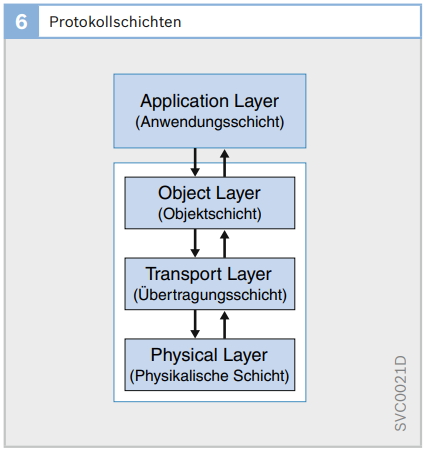
\includegraphics[width=0.4\linewidth]{own/CAN/Protokollschichten_BBA96.png}
        \caption{Grafik Protokollschichten, Quelle: \cite{BAA2011, S.96}}
        \label{fig:Protokollschichten}
    \end{figure}

    \subsection{Adressierung}
    Der CAN-Bus arbeitet mit der inhaltsbezogenen Adressierung, bei der eine einzelne Nachricht einen Identifier bekommt.
    Dieser Identifier besteht aus 11 Bit bei einem Standard-Format-Identifier und 29 Bit beim Extended-Format-Identifier.
    Mit dem 29 Bit Identifier ist es möglich, über 536 Millionen ($2^{11}$) unterschiedliche CAN-Botschaften in einem System zu übertragen, während mit dem 11 Bit Identifier nur circa 2000 ($2^{9}$) Nachrichten übertragen werden können.
    Im weiteren Verlauf betrachten wir allerdings nur den 11 Bit Identifier.

    \subsection{Steuerung des Zugriffs}
        \subsubsection{Priorisierung}
        Um eine reibungslose Kommunikation mit dem Multimaster Prinzip zu ermöglichen, müssen manche Botschaften vor anderen priorisiert werden.
        Dies wird über den Identifier gelöst, wobei ein Identifier mit niedriger Binärzahl für eine hohe Priorität und ein Identifier mit hoher Binärzahl für eine niedrige Priorität steht.
        Die Vergabe der Priorität wird anhand von der Änderungsgeschwindigkeit oder der Sicherheitsbedeutung einer Nachricht bestimmt.

        \subsubsection{Arbitrierungsphase}
        Befindet sich der Bus im rezessiven Zustand (der Bus ist frei), kann jede Station mit dem Senden beginnen.
        Die übermittelte Nachricht startet mit einem dominanten Bit, in dessen Anschluss der Identifier übertragen wird.
        Sobald mehrere Stationen gleichzeitig anfangen auf den Bus zu senden, setzt sich die Nachricht mit der höchsten Priorität durch, wodurch es zu keinem Zeit- und Datenverlust kommt.
        Jede Station, die ein rezessives Bit sendet, wird durch ein dominantes Bit, dass von einer anderen Station gesendet wird, überschrieben.
        Die Sendestationen prüfen mit einem Logischen UND, ob der Pegelstatus, mit dem von ihnen gesetzten übereinstimmt.
        Ist dies nicht der Fall, bricht die Botschaft ihre Nachricht ab, weshalb sich die Botschaft mit der höchsten Priorität durchsetzt.
        Alle anderen Sender warten nun, bis der Bus wieder frei ist und beginnen erneut mit dem Senden.
        Um Konflikte des Überschreibens vorzubeugen, dürfen zwei Nachrichten niemals denselben Identifier besitzen.
        Bei CAN2.0A muss die Nachricht mit der höchsten Priorität 130 Bitzeiten warten, was bei einer Datenübertragungsrate von $500kBit/s$ etwa eine Verzögerung von $260 \mu s$ ergibt.
        Wird die Busauslastung allerdings höher, erhöht sich der zeitliche Versatz von Nachrichten mit niedriger Priorität stark.
        Man kann nicht sicher sein, ob die Nachricht überhaupt ankommt, weshalb das Bussystem auf die einzelnen Gegebenheiten abgestimmt sein muss. 
        
        \begin{figure}[!htbp]
            \centering
            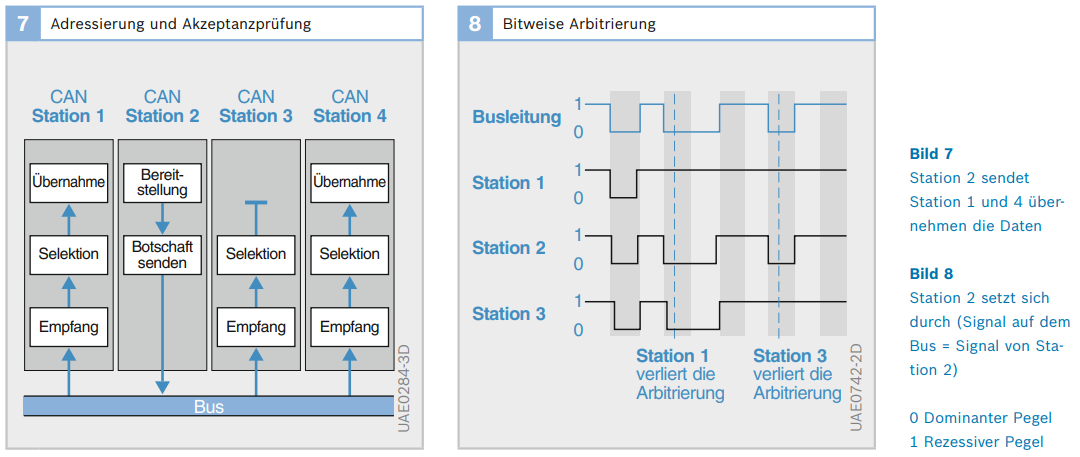
\includegraphics[width=0.7\linewidth]{own/CAN/AdressierungArbitrierung_BAA97.png}
            \caption{Grafik Adressierung, Akzeptanzprüfung, Bitweise Arbitrierung, Quelle: \cite{BAA2011, S.97}}
            \label{fig:AdressierungArbitrierung}
        \end{figure}


    \subsection{Botschaftsformat}
        \subsubsection{Arten der Telegrammformate}
        Zum einen gibt es das Data-Frame (Datentelegramm), in dem Nachrichten, die von einer sendenden Station bereitgestellt werden, gesendet werden.
        Ein störungsfreies Netzwerk kommt ausschließlich mit dieser Telegrammart aus.
        Mit dem Remote-Frame (Datenanforderungstelegramm) kann eine Station benötigte Daten von einer Datenquelle anfordern.
        Die Datenquelle sendet dann mit entsprechenden Daten.
        Bei CAN wird dies nur recht selten eingesetzt, da die Datenquelle selbst in bestimmten Zeitabständen die Daten unaufgefordert sendet.
        Ein Error-Frame (Fehlertelegramm) wird gesendet, wenn eine Station einen Fehler erkennt, um den anderen Stationen diesen Fehler mitzuteilen.
        Zuletzt gibt es noch das Overload-Frame (Überlastungstelegramm), bei dem eine Station den anderen mitteilt, dass er zum jetzigen Zeitpunkt keine weiteren Frames verarbeiten kann, da er überlastet ist.
        Es gibt mit CAN2.0A und CAN2.0B zwei Möglichkeiten einen Frame aufzubauen, wobei im weiteren Verlauf nur CAN2.0A betrachtet wird. 

        \subsubsection{Frames}
        \begin{figure}[!htbp]
            \centering
            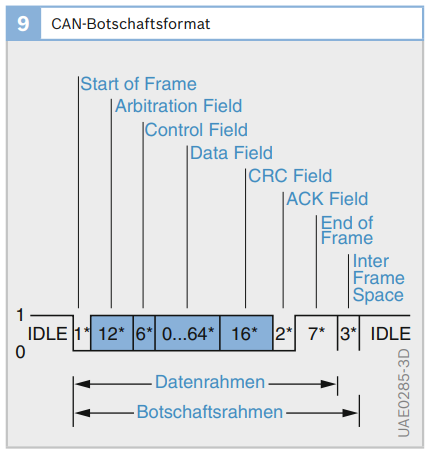
\includegraphics[width=0.4\linewidth]{own/CAN/Botschaftsformat_BAA98.png}
            \caption{Grafik CAN-Botschaftsformat, Quelle: \cite{BAA2011, S.98}}
            \label{fig:Botschaftsformat}
        \end{figure}

            \paragraph{Start-Of-Frame}
            Ein Frame wird mit dem Start-Of-Frame eingeleitet, indem ein dominantes Bit als Start der Übertragung dient.
            Hierdurch werden alle Knoten synchronisiert und CAN braucht keine Uhr, um die Knoten zu synchronisieren. 

            \paragraph{Arbitration Field}
            Danach beginnt das Arbitration Field.
            Bei CAN2.0A wird der 11Bit Identifier mit einem Kontrollbit und einem RTR-Bit (Remote Transmission Request Bit) gesendet.
            Das RTR-Bit sagt aus, ob das Frame ein Data- oder Remote-Frame ist.
            Ein Data-Frame wird durch ein dominantes RTR-Bit und ein Remote-Frame durch ein rezessives Bit dargestellt.
            Wenn eine Station sendet, während die andere Station eine Nachricht anfragt, also beide denselben Nachrichtenidentifier senden, wird der Konflikt über das RTR-Bit gelöst und die Sendestation sendet die Daten, während die Requeststation diese empfängt. 

            \paragraph{Control Field (Kontrollfeld)}
            Das Kontrollfeld besteht aus einem IDE-Bit (Identifier Extension Bit), welches bei CAN2.0A dominant und bei CAN2.0B rezessiv gesendet wird.
            Dieses Bit ist gefolgt von einem rezessiven Bit, dass für die Zukunft reserviert ist.
            Außerdem werden im Control Field noch vier Bits gesendet, die die Anzahl der Datenbytes im Datenfeld beschreibt, um eine Datenprüfung durchführen zu können.

            \paragraph{Data Field (Datenfeld)}
            Das Datenfeld enthält Daten zwischen 0 und 8 Bytes.
            Es ist auch möglich, mehrere Botschaften in einer Nachricht und in einem Datenfeld zu übertragen.
            Die kürzeste mögliche Nachricht besitzt 0 Bytes und trägt somit keine Daten, und wird deshalb gerne zum Synchronisieren verteilter Prozesse verwendet.
            Der gesendete Frame hätte in diesem Fall eine Größe von nur 44 Bit. 

            \paragraph{CRC Field (Sicherungsfeld)}
            Im Cyclic-Redundancy-Check-Field (zyklisches Redundanzprüfungsfeld) wird eine, vom Data-Field berechnete, 15 Bit Prüfsumme gesendet und mit einem 16. rezessiven Bit abgeschlossen.
            Das CRC-Field dient zur Erkennung von auftretenden Übertragungsstörungen.

            \paragraph{ACK Field (Quittierungsfeld)}
            Mit dem ACK-Field (Acknowledgement- oder Bestätigungsfeld) wird von einem Knoten, direkt im Anschluss an das Data Field, der erfolgreiche Empfang einer Nachricht bestätigt.
            Dieser Knoten muss die Daten nicht empfangen, sondern teilt dem Sender lediglich mit, dass die Nachricht korrekt gesendet wurde.
            Das ACK-Field wird vom Sender rezessiv gesendet und bei erfolgreichem Empfang eines Empfängers dominant überschrieben. 

            \paragraph{End of Frame (End-Kennung)}
            Die End-Kennung kennzeichnet das Ende einer Botschaft mit sieben rezessiven Bits. 

            \paragraph{Inter Frame Space (Rahmsubsubsubsection)}
            Die Rahmenpause besteht aus drei rezessiven Bits und signalisiert einen wieder freien Bus.
            Dies wird allerdings von Error- und Overload-Frames nicht beachtet, sodass diese direkt senden können.
            Dadurch wird eine direkte Signalisierung von Fehlern und Problemen ermöglicht.

    \subsection{Störungserkennung}
    Es kann nie von einer störungsfreien Datenübertragung ausgegangen werden.
    Allerdings ist eine sichere und zuverlässige Datenübertragung für sicherheitsrelevante Bauteile im Automobil vonnöten, weshalb es die Möglichkeit geben muss, die Datenübermittlung auf Korrektheit zu überprüfen.
    Dafür bietet CAN mehrere Prüfmechanismen an.
    Bei der zyklische Redundanzprüfung berechnet ein Algorithmus eine Prüfsumme, die mit der Nachricht übermittelt wird.
    Der Empfänger rechnet diese ebenfalls aus und vergleicht diese mit der gesendeten.
    So kann entschieden werden, ob die Nachricht erfolgreich übermittelt wurde.
    Mit dem Frame-Check (Rahmenformat-Überprüfung) prüfen alle Busteilnehmer, ob die gesendeten oder empfangenen Datenrahmen die vorgegebenen Datenrahmengrößen einhalten.
    Mit dem ACK-Check bestätigt eine andere Station den korrekten Empfang einer Nachricht mit einem ACK-Bit.
    Beim Monitoring überwacht der Sender fortlaufend den Buspegel und ist somit in der Lage, Übertragungsfehler eigenständig zu identifizieren.
    Die Bitstuffing Prüfung wird verwendet, um zu schauen, ob zwischen Start-of-Frame und dem Ende des CRC-Field maximal fünf aufeinanderfolgende Bits den identischen Zustand besitzen.
    Der Sender fügt nach fünf identischen Bits ein Bit in entgegengesetztem Zustand ein, um mit der Bitstuffing Prüfung konform zu sein.
    Diese Zusatzbits werden, beim sogenannten Destuffing, vom Empfänger beim Empfang wieder gelöscht. 
    Damit ist erkennbar, ob eine Leitungsstörung vorliegt, und das Synchronisieren zwischen Knoten lässt sich durch einen garantierten wechseln der Zustände einfacher lösen. 

        \subsubsection{Error Frames}
        Wird ein Fehler von einem Knoten erkannt, sendet dieser einen Error-Frame, der aus 6 Dominanten Bits besteht.
        Dadurch wird erreicht, dass Bitstuffing erkannt wird und alle anderen Knoten auch einen Error Frame mit 6 dominanten Bits senden.
        Ein Error-Frame wird mit 8 rezessiven Bits abgeschlossen.

        \subsubsection{Fehlererkennung bei Ausfällen}
        Defekte Stationen können den Busverkehr stark belasten und stören, wenn diese häufig fehlerhafte Botschaften senden oder korrekte Botschaften durch das Senden eines Error-Frames unterbrechen.
        Deshalb ist es mithilfe einer statistischen Fehlerauswertung möglich, den Fehler zu lokalisieren.
        Die Station erkennt die Wahrscheinlichkeit ihrer eigenen Fehlfunktion daran, wie häufig sie Botschaften abbricht, bevor andere Stationen ein Error-Frame senden.
        Beim Erkennen der eigenen Fehlfunktion bricht die Station ihre Kommunikation selbstständig ab. 

\section{Hardware}
    \subsection{CAN-Controller}
    Der CAN-Controller erzeugt aus zu übertragenden Daten einen Frame mit allen für das CAN-Protokoll erforderlichen Felder. 

        \subsubsection{Basic-CAN}
        Mit einem Basic-CAN Controller ist es nur möglich die Grundfunktionen eines CAN-Protokolls zur Erzeugung des Bitstroms zu realisieren.
        Dadurch ist dieser kostengünstiger und braucht eine kleinere Chipfläche.
        Allerdings steht nur ein Zwischenpuffer zur Verfügung, auf den ein Rechner (z.B. ein Mikroprozessor) zugreift und der Rechner muss die Daten aus dem Puffer gelesen haben, bevor der CAN-Controller neue Daten empfangen kann.
        Auch die Akzeptanzprüfung muss vom Rechner durchgeführt werden, weshalb dieser die Rechenkapazitäten für die CAN-Verwaltung zur Verfügung stellen muss.
        Deshalb wird Basic-CAN meist nur für niedrige Übertragungsraten oder für hohe Übertragungsraten mit wenigen Nachrichten verwendet.  

        \subsubsection{Full-CAN}
        Ein Full-CAN Controller bearbeitet alle Akzeptanztests und regelt die Sende- und Empfangssteuerung.
        Dieser bekommt die zu akzeptierenden Nachrichten beim Initialisieren mitgeteilt und leitet nur noch diese bestimmten Nachrichten an den angeschlossenen Rechner weiter.
        Diese Art von CAN-Controllern ist meist schon auf Chips integriert, da dies günstigere Herstellungskosten mit sich bringt. 
        
        \begin{figure}[!htbp]
            \centering
            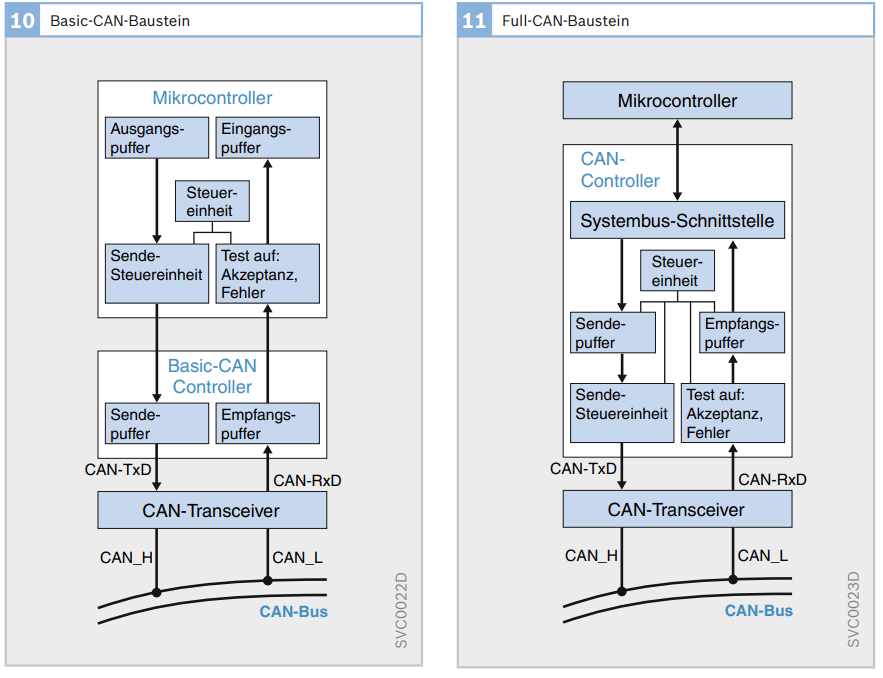
\includegraphics[width=0.5\linewidth]{own/CAN/HardwareCAN_BAA102.png}
            \caption{Grafik Basic-CAN und Full-CAN Baustein, Quelle: \cite{BAA2011, S.102}}
            \label{fig:HardwareCAN}
        \end{figure}

        \subsubsection{Bauteile ohne lokalen Rechner}
        Es gibt auch CAN-Bauteile ohne lokalen Rechner, die Daten nur über Ports ein und auslesen können.
        Dies ist geeignet für Sensoren und Aktoren, da diese Art der Anbindung an CAN günstiger ist.
        Allerdings wird hierfür ein Master-Knoten benötigt, um sie zu steuern. 

    \subsection{Transceiver}
    Ein Transceiver regelt aus dem vom CAN-Controller erzeugten Bitstrom die richtigen Spannungspegel, die für den CAN-Bus notwendig sind.
    Bei einem Zweidrahtleitungssystem sind dies CAN\_H, CAN\_L und die Referenzspannung $U_{ref}$. 

    \subsection{Sleep Mode}
    Der CAN-Bus muss auch bei ausgeschalteter Zündung betriebsbereit sein.
    Um das Bordnetz möglichst wenig zu belasten, können CAN-Bauteile in einen Sleep-Mode verfallen.
    Im Sleep-Mode wird der Sendeteil eines Transceivers ausgeschaltet, um den Stromverbrauch zu senken, während der Empfängerteil aktiv bleibt, um den Bus zu beobachten, ob eine Nachricht, wie z.B. eine Wake-Up Botschaft übertragen wird. 

\section{Erweiterungen von CAN und Protokolle auf CAN-Basis}
Dass der CAN-Bus ein sehr beliebtes Übertragungsmedium ist, sieht man an den vielzähligen Abwandlungen vom originalen CAN und dem großen Einsatzbereich außerhalb der Automobilbranche. 

    \subsection{CAN FD}
    Da eine Bandbreitenerweiterung von CAN2.0 erwünscht wurde, entwickelte die Robert Bosch GmbH 2012 den CAN FD (CAN Flexible Data Rate) Standard.
    Ein CAN-FD System kann sowohl CAN-FD Nachrichten als auch normale CAN-Nachrichten korrekt interpretieren.
    Allerdings kann ein normales CAN2.0 System keine CAN FD Nachrichten interpretieren.
    Damit nun CAN-FD Steuergeräte mit CAN-FD Steuergeräten mit bis zu 1Mbit/s Daten austauschen können, werden die CAN2.0 Steuergeräte temporär vom Bus genommen und die CAN FD Steuergeräte umgeschaltet, sodass sie bis zu 64 Datenbytes verarbeiten können.
    Dies wird durch ein zusätzliches Umschaltbit umgesetzt. 

    \subsection{CAN XL}
    Als Forderungen nach einer erneuten Bandbreitenerhöhung beim CAN-Bus laut wurden, wurde CAN XL entwickelt, um ein Datenfeld von 2048 Bytes und eine Datenrate von bis zu 10MBit übertragen zu können.
    Dies ermöglicht Ethernet Pakete, die immer mehr Einzug in das moderne Fahrzeug finden, zu tunneln.
    CAN XL ist auch kompatibel mit CAN FD und CAN2.0, allerdings schaltet CAN XL, bei der Datenübertragung, auf eine andere physikalische Ebene mit unterschiedlichen Datenraten, Spannungen und optional auch einer unterschiedlichen Pulsweitenmodulation um. 

    \subsection{Andere CAN-Protokolle}
        \subsubsection{CAN TP2.0}
        Mit dem CAN-Transportprotokoll 2.0 wurde von VW ein Transportprotokoll eingeführt, dass speziell zu Diagnosezwecken entwickelt wurde.
        Es wird möglich mehr als 8 Daten Bytes in mehreren CAN-Nachrichten zu übertragen, während derselbe Identifier verwendet wird.
        Dadurch müssen mehrere zusammengehörige Datenpakete nicht mehr einzeln aufgefordert werden, was eine effizientere Diagnosekommunikation erlaubt. 

        \subsubsection{Bosch MCNet}
        Mit dem Bosch MCNet (Mobile Communication Network) wurde ein Transportprotokoll auf physikalischer Ebene und Sicherungsschicht entwickelt, welches speziell für Multimedia-Anwendungen angepasst war.
        MCNet kann nur Befehle und Informationen transportieren, allerdings keine Video- und Audio-Dateien.
        Dadurch setzte es sich nie durch, zeigt aber trotzdem das Potential und die Weiterentwicklungsfähigkeit, die CAN aufweist.  
        
        \subsubsection{CANopen}
        In der Automobilindustrie gibt es, anders als in der Automatisierungstechnik, fast keine Standardisierung für die Anwendungsschicht bei CAN.
        CANopen standardisiert die Anwendungsschicht und wird hauptsächlich für standardisierte Anwendungsprofile in Fahrzeugen genutzt.
        Beispiele hierfür wären Kommunalfahrzeuge mit Anbaugeräten oder der Umbau von Serienfahrzeugen zu Sonderfahrzeugen. 
        \newline\newline
        Für mehr Informationen zu weiteren CAN-Protokollen, CAN FD und CAN XL Quelle \cite{KIA2022}.